%-------------------------
% Resume in Latex
% Author : Sourabh Bajaj
% License : MIT
%------------------------

\documentclass[letterpaper,11pt]{article}

\usepackage{latexsym}
\usepackage[empty]{fullpage}
\usepackage{titlesec}
\usepackage{marvosym}
\usepackage[usenames,dvipsnames]{color}
\usepackage{verbatim}
\usepackage{enumitem}
\usepackage[hidelinks,pdftex]{hyperref}
\usepackage{fancyhdr}

% footnote to the bottom
\usepackage[bottom]{footmisc}

% currency symbols
\usepackage{textcomp}

% image insertion
\usepackage{graphicx}

% floating-point calculation for currency
\usepackage{fp}

\usepackage{numprint}

%%
\def \includeMinor {}

% Blank term definition
%\def \disallowBlankTerm {}

% Currency definition.
% comment below definition in order to use dollar currency
%\def \currencyEuro {}
%\def \currencyPound {}
%\def \currencyCanadaDollar{}
%\def \currencySwissFranc{}

% thousand separator
\ifx \currencyEuro \undefined
  \ifx \currencyPound \undefined
    \ifx \currencyCanadaDollar \undefined
      \ifx \currencySwissFranc \undefined
          % currencyDollar
          \npthousandsep{,}\npthousandthpartsep{}\npdecimalsign{.}
          \def \symbolcurrency {\textdollar}
          \def \textcurrency {USD}
          \def \rateWonCurrency {1122.90}
          \def \dateCurrency {(Feb 23, 2019)}
      \else
        % currencySwissFranc
          \npthousandsep{'}\npthousandthpartsep{}\npdecimalsign{.}
          \def \symbolcurrency {CHF\ }
          \def \textcurrency {CHF}
          \def \rateWonCurrency {1121.61}
          \def \dateCurrency {(30 Jan, 2019)}
      \fi
    \else
          % currencyCanadaDollar
          \npthousandsep{,}\npthousandthpartsep{}\npdecimalsign{.}
          \def \symbolcurrency {\textdollar}
          \def \textcurrency {CAD}
          \def \rateWonCurrency {845.18}
          \def \dateCurrency {(Dec 7, 2018)}
    \fi
  \else
    % currencyPound
    \npthousandsep{,}\npthousandthpartsep{}\npdecimalsign{.}
    \def \symbolcurrency {\textsterling}
    \def \textcurrency {GBP}
    \def \rateWonCurrency {1450.36}
    \def \dateCurrency {(19 Jan, 2019)}
  \fi
\else
  % currencyEuro
  \npthousandsep{.}\npthousandthpartsep{}\npdecimalsign{,}
  \def \symbolcurrency {\texteuro}
  \def \textcurrency {EUR}
  \def \rateWonCurrency {1282.47}
  \def \dateCurrency {(13 Dec, 2017)}
\fi

% acceptance rate colour
\definecolor{acceptance}{RGB}{78, 129, 189}

\pagestyle{fancy}
\fancyhf{} % clear all header and footer fields
\fancyfoot{}
\renewcommand{\headrulewidth}{0pt}
\renewcommand{\footrulewidth}{0pt}

% Adjust margins
\addtolength{\oddsidemargin}{-0.375in}
\addtolength{\evensidemargin}{-0.375in}
\addtolength{\textwidth}{1in}
\addtolength{\topmargin}{-.5in}
\addtolength{\textheight}{1.0in}

\urlstyle{same}

\raggedbottom
\raggedright
\setlength{\tabcolsep}{0in}

% Sections formatting
\titleformat{\section}{
  \vspace{-4pt}\scshape\raggedright\large
}{}{0em}{}[\color{black}\titlerule \vspace{-5pt}]

%-------------------------
% Custom commands
\newcommand{\resumeItem}[2]{
  \item\small{
    \textbf{#1}{: #2 \vspace{-2pt}}
  }
}

\newcommand{\resumeSimpleItem}[1]{
  \item\small{
    {#1 \vspace{-2pt}}
  }
}

\newcommand{\resumeSubheading}[4]{
  \vspace{-1pt}\item
    \begin{tabular*}{0.97\textwidth}{l@{\extracolsep{\fill}}r}
      \textbf{#1} & #2 \\
      \textit{\small#3} & \textit{\small #4} \\
    \end{tabular*}\vspace{-5pt}
}

\newcommand{\resumeSubItem}[2]{\resumeItem{#1}{#2}\vspace{-4pt}}

\renewcommand{\labelitemii}{$\circ$}

\newcommand{\resumeSubHeadingListStart}{\begin{itemize}[leftmargin=*]}
\newcommand{\resumeSubHeadingListEnd}{\end{itemize}}
\newcommand{\resumeItemListStart}{\begin{itemize}}
\newcommand{\resumeItemListEnd}{\end{itemize}\vspace{-5pt}}
\newcommand{\resumeHeadItemListStart}{\begin{itemize}[leftmargin=*]}
\newcommand{\resumeHeadItemListEnd}{\end{itemize}\vspace{-5pt}}

%-------------------------------------------
%%%%%%  CV STARTS HERE  %%%%%%%%%%%%%%%%%%%%%%%%%%%%


\begin{document}

\begin{minipage}[l]{0.33\textwidth}
 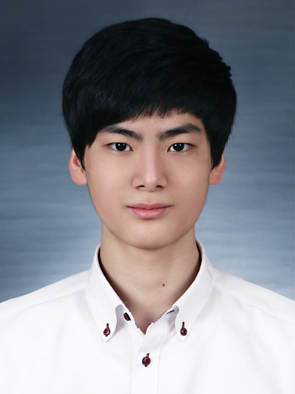
\includegraphics[scale=0.3]{Kiyoon.jpg}
  \vspace{2mm}
\end{minipage}
\begin{minipage}[r]{0.55\textwidth}
 Hello, I'm a computer scientist with computer vision, machine learning and signal processing background.

\end{minipage}

%----------HEADING-----------------
\begin{tabular*}{\textwidth}{l@{\extracolsep{\fill}}r}
  \textbf{\href{https://kiyoon.kim/}{\Large Kiyoon Kim}} & Email : \  \href{mailto:kiyoon.kim@ed.ac.uk}{kiyoon.kim@ed.ac.uk}\\
  \href{https://kiyoon.kim/}{https://kiyoon.kim/} & Mobile : \ \ \ \ \ \  +44-7494-630465 \\
  
\end{tabular*}

%-----------EDUCATION-----------------
\section{Education}
  \resumeSubHeadingListStart
    \resumeSubheading
      {The University of Edinburgh}{Edinburgh, United Kingdom}
      {PhD in Informatics: Robotics, Computer Vision, Computer Graphics and Animation}{Sep 2019 -- Aug 2023 (Estimated)}
    \resumeSubheading
      {The University of Edinburgh}{Edinburgh, United Kingdom}
      {MSc in Artificial Intelligence}{Sep 2018 -- Aug 2019}
    \resumeSubheading
      {Ulsan National Institute of Science and Technology (UNIST)}{Ulsan, South Korea}
      {Bachelor in Electrical Engineering, Computer Science and Engineering: \textbf{magna cum laude}}{Mar 2014 -- Feb 2018}
      \resumeItemListStart
        \resumeItem{Contribution Award\footnotemark}
          {Chairman's Award}
        \resumeItem{GPA of major subjects}
          {\numprint{4.00}/\numprint{4.3} (\numprint{96.0}/100)}
        \resumeItem{Total Grade Point Average}
          {\numprint{3.79}/\numprint{4.3} (\numprint{93.9}/100)}
      \resumeItemListEnd
  \resumeSubHeadingListEnd
  
  \footnotetext{Students who have shown especially good behaviour or enhanced the university's honour can be given a contribution award. The contribution award winner shall be selected by deliberation of the Committee based on recommendations from the head of the school (department) in each school (department). In 2018, among 704 undergraduates from various departments, 6 people have been awarded.}

%-----------SCHOLARSHIPS-----------------
% \newcommand{\calcCurrencyPrice}[2]{\FPeval{#2}{round(#1 / \rateWonCurrency,0)}} % #1 = input, #2 = output
% \newcommand{\setWonPrice}[1]{\def\wonprice{#1}\calcCurrencyPrice{\wonprice}{\currencyprice}}   % Define won price and calculate currency price from the won price
% \def \currencyWonPrint{\textwon\numprint{\wonprice} (\symbolcurrency\numprint{\currencyprice})}

% \section{Scholarships}
% Currency measure: 1 \textcurrency{} = \numprint{\rateWonCurrency} KRW \dateCurrency{}
%   \resumeSubHeadingListStart
%     \resumeSubheading
%       {NAVER UNIST Undergraduate Poster Award (NAVER UUPA)}{NAVER Corp., UNIST}
%       {\setWonPrice{2500000}\currencyWonPrint}{Dec 2017}
%     \resumeSubheading
%       {UC Berkeley Entrepreneurship Programme}{UNIST}
%       {\setWonPrice{9975200}\currencyWonPrint}{Jan 2017 -- Mar 2017}
%     \resumeSubheading
%       {Living Scholarship}{UNIST}
%       {\setWonPrice{2140000}\currencyWonPrint}{Mar 2016 -- Dec 2017}
%     \resumeSubheading
%       {Allowance}{UNIST}
%       {\setWonPrice{2517600}\currencyWonPrint}{Mar 2016 -- Dec 2017}
%     \resumeSubheading
%       {National Science \& Engineering Scholarship}{Korea Student Aid Foundation}
%       {\setWonPrice{12588000}\currencyWonPrint}{Mar 2016 -- Dec 2017}
%     \resumeSubheading
%       {Korea Supercomputing Challenge (KSC 2015)}{KISTI Supercomputing Education Center}
%       {\setWonPrice{500000}\currencyWonPrint{} (shared by 2 members)}{Oct 2015}
%     \resumeSubheading
%       {HeXATHON}{UNIST, NAVER Corp.}
%       {\setWonPrice{1500000}\currencyWonPrint{} (shared by 4 members)}{May 2015}
%     \resumeSubheading
%       {Tutoring for Engineering Programming I (3 semesters)}{UNIST}
%       {\setWonPrice{1200000}\currencyWonPrint}{Sep 2014 -- Dec 2015}
%     \resumeSubheading
%       {Academic Performance Scholarship}{UNIST}
%       {\setWonPrice{12660000}\currencyWonPrint}{Mar 2014 -- Dec 2015}
%   \resumeSubHeadingListEnd

%-----------PUBLICATION----------------
\section{Publications}
  \resumeHeadItemListStart
    \resumeSimpleItem
          {M. S. Ryoo, \underline{K. Kim} and H. J. Yang, ``Extreme Low Resolution Activity Recognition with Multi-Siamese Embedding Learning,'' \textit{AAAI Conference on Artificial Intelligence}, New Orleans, Louisiana, February 2018. \textit{{\color{acceptance}{[acceptance rate: 24.6\%]}}}\\
          \href{https://arxiv.org/pdf/1708.00999.pdf}{\underline{https://arxiv.org/pdf/1708.00999.pdf}}}
    \resumeItem{Patent}{Falling out of hair management system\\
                      \href{https://patents.google.com/patent/KR20140094301A/en}{\underline{https://patents.google.com/patent/KR20140094301A/en}}}
  \resumeHeadItemListEnd

%-----------EXPERIENCE-----------------
\section{Experience}
  \resumeSubHeadingListStart
    \resumeSubheading
      {Demonstration for Machine Learning Practical}{The University of Edinburgh}
      {Ran lab sessions for the Machine Learning Practical (MSc module).}{Sep 2019 --}
      
    \resumeSubheading
      {Tutoring for Object-Oriented Programming}{The University of Edinburgh}
      {Ran 2 tutorial sessions of OOP Java programming tutorials with Eclipse IDE.}{Jan 2019 -- Apr 2019}
      \resumeItemListStart
        \resumeSimpleItem{Nominated for the \textbf{Best Student Who Tutors Award}}
      \resumeItemListEnd
      
    \resumeSubheading
      {Tutoring for Imperative Programming}{The University of Edinburgh}
      {Ran tutorial sessions of Java programming with Greenfoot IDE.}{Nov 2018}
      
    \ifdefined \includeMinor
    \resumeSubheading
      {Private Tutoring}{Personal}
      {Tutored TOEIC (English) to a job seeker.}{Jul 2018 -- Aug 2018}
    \fi
      
    \ifdefined \includeMinor
    \resumeSubheading
      {Private Tutoring}{Personal}
      {Tutored R Language to a master student.}{Apr 2018}
    \fi
    
    \resumeSubheading
      {NAVER UNIST Undergraduate Poster Award (NAVER UUPA)}{NAVER Corp., UNIST}
      {Poster presentation of Extreme Low Resolution Activity Recognition: won \textbf{1st place}}{Dec 2017}
    \resumeSubheading
      {EgoVid Inc. (\href{http://egovid.com}{http://egovid.com})}{Ulsan, South Korea}
      {Machine Learning Researcher \& Developer}{May 2016 -- Dec 2017}
      \resumeItemListStart
        \ifdefined \includeMinor
        \resumeItem{Drone Project Manager}
          {Autonomous drone project using ROS on NVIDIA Jetson TX2 embedded board.}
        \fi
        \resumeItem{Realtime Demonstration Running on Embedded Device at CVPR 2017}
          {Demonstrated my work running on NVIDIA Jetson TX2 and helped my colleague for implementing different demonstration about Video Anonymisation Algorithm at CVPR (Computer Vision Pattern Recognition) 2017 conference.\\
          \href{https://youtu.be/7jkSum_pj9o?t=25s}{\underline{https://youtu.be/7jkSum\_pj9o?t=25s}}}
        \resumeItem{UC Berkeley Entrepreneurship Programme}
          {Visited UC Berkeley Sutardja Center of Entrepreneurship \& Technology for 9 weeks to exchange ideas about making a start-up company.\\
          UC Berkeley News Article: \href{http://scet.berkeley.edu/keeping-personal-machine-learning-meets-egovid}{\underline{http://scet.berkeley.edu/keeping-personal-machine-learning-meets-egovid/}}}
        \resumeItem{Attended Conferences}
          {AAAI Conference on Artificial Intelligence 2017, San Francisco, California, USA\\
          Asilomar 2016, Pacific Grove, California, USA\\
          Ubicomp 2016, Heidelberg, Germany}
          
        \ifdefined \includeMinor
        \resumeItem{Linux GPU Computing Server Setup for Machine Learning}
          {Installed Ubuntu Server and programs needed for machine learning and sharing devices with multiple users. VNC remote desktop, Docker and Virtualenv.}
        \fi
          
        \ifdefined \includeMinor
        \resumeItem{Study: Machine Learning and Computer Vision}
          {Studied machine learning and computer vision with Coursera, Udacity courses.}
        \resumeItem{Study: OFDM Radar Signal Processing}
          {Studied OFDM radar signal processing for possible future work in radar classification machine learning problem.}
        \fi
      \resumeItemListEnd
    
    \ifdefined \includeMinor
    \resumeSubheading
      {Private Tutoring}{Personal}
      {Tutored Computer Science and Engineering subjects to two university students.}{Mar 2016 -- Dec 2016}
      \resumeItemListStart
        \resumeSimpleItem{Object Oriented Programming (C++)}
        \resumeSimpleItem{Data Structure (C++)}
        \resumeSimpleItem{Principles of Programming Languages (SML, Racket, Python)}
      \resumeItemListEnd
    \fi
      
    \ifdefined \includeMinor
    \resumeSubheading
      {Private Tutoring}{Personal}
      {Tutored C Language to a pre-high school student.}{Jan 2016 -- Feb 2016}
    \fi
      
    \ifdefined \includeMinor
    \resumeSubheading
      {USPTO Patent Information Crawler}{UNIST}
      {Developed in Python for building custom database.}{Dec 2015 -- Apr 2016}
    \fi
      
    \resumeSubheading
      {Korea Supercomputing Challenge (KSC 2015)}{KISTI Supercomputing Education Center}
      {MPI parallel computing competition: won \textbf{5th place}}{Oct 2015}
      
    \ifdefined \includeMinor
    \resumeSubheading
      {Intel Xeon Phi optimisation, parallelisation education}{Intel Corp.}
      {Completed the education with practices about OpenMP, Vectorisation, and Intel compiler.}{Aug 2015}
    \fi
      
    \ifdefined \includeMinor
    \resumeSubheading
      {Personal Linux Server Buildup}{Personal}
      {Fedora server buildup for personal use}{Aug 2015}
      \resumeItemListStart
        \resumeSimpleItem{File cloud \& synchronisation server}
        \resumeSimpleItem{Multimedia streaming server}
        \resumeSimpleItem{Web \& DB server (Gitlab, URL Shortener, Spam filtering)}
      \resumeItemListEnd
    \fi
      
    \ifdefined \includeMinor
    \resumeSubheading
      {WISET Startup Springboard}{UNIST}
      {Completed the entrepreneurship programme.}{Aug 2015}
    \fi
    
    \ifdefined \includeMinor
    \resumeSubheading
      {Private Tutoring}{Personal}
      {Tutored mathematics to a high school student.}{July 2015 -- Aug 2015}
    \fi
      
    \resumeSubheading
      {HeXATHON}{UNIST, NAVER Corp.}
      {QR code waiting system implemented with Raspberry Pi: won \textbf{1st place}}{May 2015}
      
    \ifdefined \includeMinor
    \resumeSubheading
      {UNIST Startup Clinic}{UNIST, NAVER Corp.}
      {Smart home app controlling electric output}{Mar 2015}
    \fi
    
    \ifdefined \includeMinor
    \resumeSubheading
      {Private Tutoring}{Personal}
      {Tutored physics to a pre-high school student.}{Jan 2015 -- Feb 2015}
    \fi
      
    \resumeSubheading
      {Tutoring for Engineering Programming I}{UNIST}
      {Ran tutorial sessions for 3 terms.}{Sep 2014 -- Dec 2015}
      
    \ifdefined \includeMinor
    \resumeSubheading
      {Private Tutoring}{Personal}
      {Tutored mathematics to a high school student.}{Jul 2014 -- Aug 2014}
    \fi
      
    \ifdefined \includeMinor
    \resumeSubheading
      {Math Tutor at Private School}{Morning of Math}
      {Problem-solving assistant for high school students}{Jul 2014 -- Aug 2014}
    \fi
      
    \ifx \disallowBlankTerm{} \undefined
    \resumeSubheading
      {Patent: Falling out of hair management system}{South Korea}
      {Hair proportion analysis algorithm implemented in CxImage and MFC.}{Jan 2013 -- Jul 2014}
    \fi
      
    \resumeSubheading
      {Korea International Science and Engineering Fair (KISEF 2012)}{National Science Museum}
      {Exhibited and Demonstrated PowerUpdater2 at Daejeon Convention Center.}{Jan 2012}
      
    \resumeSubheading
      {Korea Olympiad in Informatics (KOI 2011)}{National Information Society Agency}
      {Demonstrated PowerUpdater2: won \textbf{bronze medal}.}{Sep 2011}
      
    \resumeSubheading
      {Sparkware (\href{http://sparkware.co.kr}{http://sparkware.co.kr})}{Personal}
      {Personal Website Management (XpressEngine), Program Development (C++, MFC)}{May 2010 -- Aug 2013}
      \resumeItemListStart
        \resumeItem{PowerUpdater, PowerUpdater2}
          {An updater program that can be customised by users easily with GUI menu.}
        \resumeItem{Waviano}
          {Playing piano with keyboard using multiple music files.}
        \resumeItem{PowerRegister}
          {An customisable activation program for Windows application programmers.}
        \resumeItem{DirectoryDateName}
          {Easily make directory with name containing current date.}
        \resumeItem{Flash programs}
          {Simple Flash programs.}
          \resumeItemListEnd
          
    \ifdefined \includeMinor
    \resumeSubheading
      {Flash programming}{Personal}
      {Studied and implemented simple Flash programs.}{Nov 2004 -- Apr 2010}
      \resumeItemListStart
        \resumeSimpleItem{Elementary, middle school teachers used my programs.}
        \resumeSimpleItem{Managed a blog to release some programs.}
      \resumeItemListEnd
    \fi


  \resumeSubHeadingListEnd
    

%--------PROGRAMMING SKILLS------------
%\section{Programming Skills}
%  \resumeSubHeadingListStart
%    \item{
%       \textbf{Languages}{: Scala, Python, Javascript, C++, SQL, Java}
%      \hfill
%      \textbf{Technologies}{: AWS, Play, React, Kafka, GCE}
%    }
%  \resumeSubHeadingListEnd
  
%--------SKILLS AND KNOWLEDGE------------
\section{Skills and Knowledge}
  Deep learning, Computer vision, Signal processing, Linux server buildup, Machine integration, Web development, Product design
  
%--------LANGUAGES, FRAMEWORKS AND TOOLS------------
\section{Languages, Frameworks and Tools}
  C $\cdot \ $ C++ $\cdot \ $ Python $\cdot \ $ Linux Bash $\cdot \ $ TensorFlow / Keras (Machine learning) $\cdot \ $ MPI (Parallel programming) $\cdot \ $ CUDA (GPU parallel programming) $\cdot \ $ MATLAB $\cdot \ $ OpenCV $\cdot \ $ Git (Version control) $\cdot \ $ Docker $\cdot \ $ NVIDIA Jetson TX2 (Embedded board and Linux) $\cdot \ $ Raspberry Pi (IoT Linux) $\cdot \ $ MFC (Windows programming) $\cdot \ $ Java $\cdot \ $ HTML $\cdot \ $ PHP $\cdot \ $ MySQL / Maria DB $\cdot \ $ R $\cdot \ $ Flash action script $\cdot \ $ Processing $\cdot \ $ NXT Robot C $\cdot \ $ Xpress Engine(Website) $\cdot \ $ Wordpress(Website) $\cdot \ $ \LaTeX
  
  

%-----------LANGUAGES-----------------
%\section{Languages}
%  \resumeSubHeadingListStart
%    \resumeSubItem{English}
%      {Fluent}
%    \resumeSubItem{Korean}
%      {Native}
%    \resumeSubItem{German}
%      {Learning the basics}
%  \resumeSubHeadingListEnd
%

%-------------------------------------------
\end{document}
